\documentclass[11pt]{jsarticle}

\usepackage{SPR}

\headerSPR
\begin{document}
	\titleSPR{\number\year}{\number\month}{\number\day}{D2}{吉田 皓太郎}
%%%%%%%%%%%%%%%%%%%%%%%%%%%%%%%%%%%%%%
	\articleSPRabst
		\begin{itemize}
			\item 機械学習を用いたカップ形状の設計支援
			\item 着後形状予測のためのカップの変形解析
		\end{itemize}
		
		
	\articleSPRobj
		\begin{enumerate}
			\item 定性的な機能要求を満たせるようなカップ形状を設計できる
			\item 布の物性とカップのパターンがどのような結びつきを持っているかを調べることができる.
		\end{enumerate}
%%%%%%%%%%%%%%%%%%%%%%%%%%%%%%%%%%%%%%
% 1.前回からのノルマ
	\articleSPRitemsone
		%\begin{enumerate}
		%	\item A
		%\end{enumerate}
		
		\tableofcontents
		
		
%%%%%%%%%%%%%%%%%%%%%%%%%%%%%%%%%%%%%%
%\begin{itemize}
%	\item 新規手法について
%	\item ISFAアウトライン
%\end{itemize}
%%%%%%%%%%%%%%%%%%%%%%%%%%%%%%%%%%%%%%
% 2.具体的な成果
	\articleSPRitemstwo
	\renewcommand{\labelitemi}{$\blacktriangledown$}
%%%%%%%%%%%%%%%%%%%%%%%%%%%%%%%%%%%%%
	\section{研究進捗について}
		先週の研究成果等について報告いたします.先週は
		\begin{itemize}
			\item 設計工学会のプロット,話の流れについて
			\item これからのTodo
		\end{itemize}
		
		\subsection{設計工学会のプロット(背景・目的)について}
		緒言における設計の背景や目的を整理し,それを色々書いてみました.理想としては,荒井先生が過去に提案していた「設計意図」と「幾何情報」を統合するモデル概念のブラジャーカップ版みたいなのを想定して話を展開してみたのですが,実際どういう風にモデルを展開すればよいか,またその検証などをどうすればよいかは間に合わなさそうなので,講演のネタとしてはボツになりそうです.
		\subsubsection{【ブラジャーカップが設計されるまで】}
			ブラジャーカップの設計現場について述べる.ブラジャーカップの設計は,まずはじめに,市場調査から始まる.市場調査では,そのときのファッションの傾向やニーズなどを調査し,デザイン画と製品コンセプト(製品要求)を決定する.このデザイン画を基に,
			\begin{itemize}
				\item パタンナーは,上記の製品要求を満足するような理想的なバストの変形状態を,頭の中で考える.
				\item 次に,その三次元形状に最も近いカップ形状を想定し,それを頭の中で展開したパターン形状を想像する.その後,想像したパターン形状に「近しい」ものを,過去の製品データから選択する.
				\item その後,そのパターンを設計者の意図に近づけるように修正する.この修正されたパターン形状はあくまで設計者の経験と勘に基づいて設計されたものであるから,この段階では,設計したパターン形状を組み立てた際に,設計者の意図が正しく反映するかはわかっていない.
			\end{itemize}
			そのため,パタンナーは設計したパターンから紙模型を作成する.
			\begin{itemize}
				\item この紙模型を見て,設計者は自身が意図した機能が発現しているかを確認する.
				\item 発現が確認されない場合は,多くの場合は,紙模型とパターン形状との関係を確認しつつ,経験と勘に基づき,どのように修正するかを決定し,パターンを修正する.
			\end{itemize}
			前述したように,パターンを修正した時点では,このパターン形状が正しいものかどうかは分からないため,同じように紙模型による試作と評価を行う.以上の工程を,設計者は,自身が意図する形状を得るまで繰り返し行う.
			
			上記の流れを整理した上で,問題点をまとめると以下のようになる.
			\begin{itemize}
				\item 理想的バスト形状からカップ形状への落とし込みの複雑さ
				\item 現状では,二次元のパターン形状のみが,データとして保管されていること.また,データの保管は,二次元形状に関する情報のみであり,その設計意図(機能)の情報(ドキュメント)は保存されていない.
				\item 「近しい」の判断が間違ってしまう可能性がある(形自身が似ているというより,同じような機能の発現できるのかを判断するべき)
				\item パターンの修正法についてが経験と勘であること
				\item カップからパターンへの落とし込みが経験と勘に基づくこと
				\item 紙模型(カップ形状)と要求機能の定量的相関(どう評価する?)
				
			\end{itemize}
		\subsubsection{【設計支援システム】}
			システムによるブラジャーカップの設計支援を達成するためには,データの保管などの部分に着目し,
			\begin{enumerate}
				\item 正確に設計意図と形状が結びついた状態で保存されていること
				\item 設計意図と形状の定量的相関を把握すること.
			\end{enumerate}
			が求められる.この1番目に着目し,設計意図と形状を正確に結びつける場合にあたって,ブラジャーカップの設計特性について考察する.
			\begin{itemize}
				\item 形状表現の難しさ
				
				概念設計から基本設計への設計段階において,ブラジャーカップは,布物性による影響を考慮していない状態,つまり紙模型の状態で形の評価が行われる.その理由は,設計者の視認性と再利用性が高いことが挙げられる.ここでいう視認性とは,形状評価の行いやすいかどうかである.最終製品としてのブラジャーカップの形状は,大きく分けて2つの要素によって決定される.
				\begin{itemize}
					\item パターン形状によるもの(形状要素)
					\item 着用などによる力の作用環境によるもの(物理的要素)
				\end{itemize}
				特に,布をはじめとする変形しやすい物性を用いて作成するブラジャーカップにおいては,後者は強く意識しなければならない.つまり,ある形状に関する設計意図が満たされていない場合,それがパターン形状によるものなのか,あるいは作用環境下における布のふるまいによるものかどうかを,設計者は見極めた上で修正を考えなければならない.そのため,視認性を上げるためには,この作用環境による形状への影響をできる限り排除した状態である方が望ましい.
				
				次に,再利用性について述べる.ブラジャーカップに用いられる布地は,力学的特性よりも着心地(通気性・肌ざわり)の要素を大きく決定する.このことから,設計現場では,過去に作成したパターンを,異なった布で試作し,意図する形状へ近づけるために修正を行う場合も多い.この場合,パターンの修正は,一から設計するときよりもずっと少なくて済むことから,効率的であるとされている.
				
				以上より,本研究では,対象とする設計段階において,現状の設計現場と同じように,カップ形状を決定する要素を切り分け,この中の形状要素を研究対象とする.この形状要素は,設計段階における紙模型の作成と評価に等しいことから,形状要素はパターンを組み立てて作成する紙模型であると考える.組み立てたパターン曲面は展開可能な曲面である可展面となる.通常の曲面を保存する手法には,例えばNURBS曲面の制御点の集合によって保存する場合がある.しかし,この可展面の特性を制御点によって表現するのは難しく,また曲面の3次元形状だけでなく,パターン形状を紐づける必要がある.したがって,上記の課題を解決するような,形状モデルを構築しなければならない.
				
				\item 取り扱う機能の複雑さ?
				
				ブラジャーカップにおける機能表現は,一般的に用いられる機能表現とは異なることが挙げられる.
				
				本研究において比較対象として取り扱う機能の特性定義は次の二つに要約される.第一の特性の定義は,対象物との作用であり,物理的行為あるいは化学変化を伴う行為を表すものである.第二の特性の定義として,幾何情報やその関係情報を用いて表現される論理式で,発現が判断されるものである.
				通常の工業製品においては要求機能は,これ以上分解することのできない下位機能の組み合わせによって表現されると考えられており,下位機能については,例えば価値工学の枠組みにおいて,147個の機能記述動詞を提案されている.
				
				ブラジャーという製品の一般的な定義は,広辞苑によると
				「ブラジャーカップは,バストの形を整える製品である」と定義されている.
				定義上に存在する「整える」という行為は,価値工学の単位機能で定義されている,「囲う」と「押さえる」という二つの単位機能に分解することができる.しかしながら,ブラジャーカップの設計現場においては,このような物理的現象に基づく機能は大きく変更されることがないため,前提条件として扱われており,設計現場ではほとんど意識されることがない.それよりも,「どのように」囲っている,押さえているのかが重要視する.詳しく述べると,「ブラジャーカップの」設計者が共有する機能は,物理的行為に基づく作用は同一であるが,作用する「度合」によって,異なる機能を持っていると認識している.形状と設計意図を結びつける研究例は種々存在しており,中でも,荒井らは,「全ての製品機能がふるまいの挙動に分解できるならば,それに対応する幾何情報と結びつけることができる」と述べている.一方,ブラジャーカップの場合には,その設計意図モデルだけでは不十分で,機能が発現している「度合」情報があって初めて,その時の幾何情報とを結びつけることが重要である.
			\end{itemize}
		以上より,上記の課題を解決し,設計意図を考慮したカップのモデリング概念が提案できれば,設計効率化につながるのではないかと考えられる.(1番目の要求)
		
		さらに,このモデリング概念を機械学習により学習することで,機能の「度合」と幾何情報の定量的関係を求めることができるのではないかと考えられる.(2番目の要求)
		\subsection{カップの形状表現についてUpdate}
			先々週に記載した,特徴量の件についてです.先々週では,第一基本量および第二基本量が下記の通りに表されることから,$ \omega_{\xi},\omega_{\eta},\omega_{\zeta},\alpha ,D$の特徴関数をいくつかの特徴量を変換し,それらを読み込めばよいとしました.
			\begin{eqnarray}
			E &=& (\alpha'+\lambda)^2 t^2 -2\cos \alpha(\alpha'+\lambda) t + 1,\\
			F &=& -\sin \alpha,\\
			G &=& 1,
			\end{eqnarray}
			
			\begin{eqnarray}
			L &=& -\omega_{\xi}+t\{\lambda(-\omega_{\xi}\cos \alpha + \omega_{\zeta}\sin \alpha)+\omega_{\zeta}'\cos \alpha + \omega_{\xi}'\sin \alpha \},  \\
			M &=& \omega_{\xi}\sin \alpha + \omega_{\zeta} \cos \alpha,  \\
			N &=& 0. 
			\end{eqnarray}
			これに加え,ワイヤーの曲率$ \kappa $が与えられている状態である場合,関係式より$ \omega_{\xi} = \sqrt{\kappa^2 - \omega_{\eta}^2} $であるため,さらに特徴関数を減らすことができ,より少ないパラメータ数で学習できると思われる.
		\subsection{これからのTodo}
			\begin{itemize}
				\item 機械学習のプログラム
				\item ガウス過程回帰をもう少し調べるorニューラルネットワークの回帰についてもう少し考える.
			\end{itemize}
		
			\begin{figure}
				\centering
				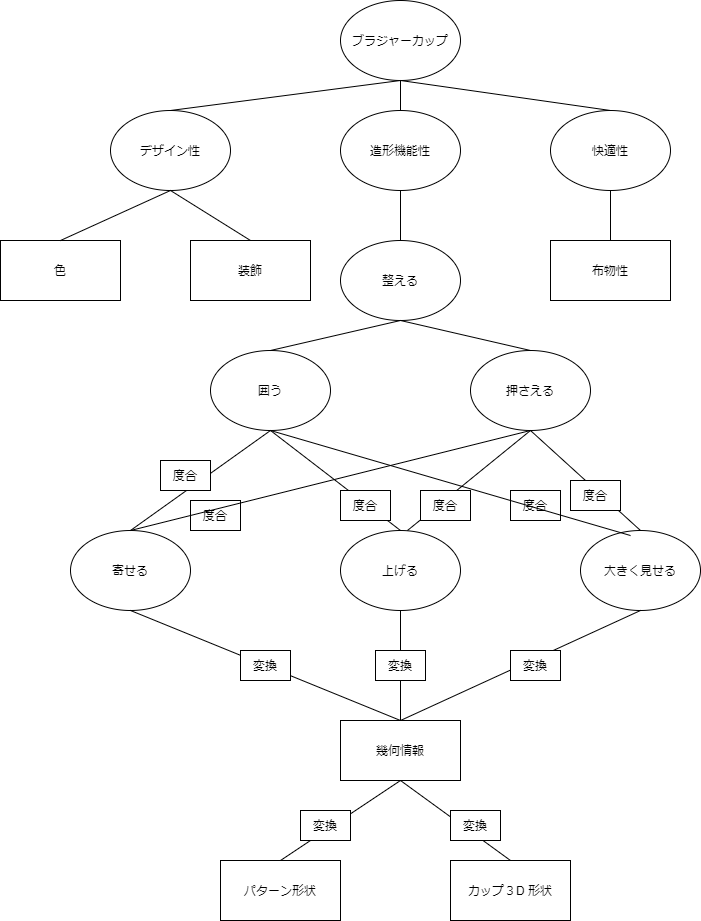
\includegraphics[scale=0.45]{./figure/BrassiereOntrogy.png}
				\caption{ブラジャーカップの概念図(参考)}
			\end{figure}
	\newpage
\vspace{10cm}
%%%%%%%%%%%%%%%%%%%%%%%%%%%%%%%%%%%%%%
% 3.達成できなかったこととその問題点
	%\articleSPRthree
%%%%%%%%%%%%%%%%%%%%%%%%%%%%%%%%%%%%%%

\vspace{14cm}
%%%%%%%%%%%%%%%%%%%%%%%%%%%%%%%%%%%%%%
	\articleSPRfour
	\articleSPRfive
\end{document}
